%LTeX: language=it
\chapter{Lezione 26/03/2020}
\section{Soglia di una reazione}
Discutiamo ora le reazioni che possono avvenire solo superando la cosiddetta
\textbf{soglia di reazione}.

Dall'equazione \ref{eq:modulo_quadro_impulso}, poiché
$\abs{\vec{p}^{\,\ast}}^2$ è una quantità positiva, allora dovrà
necessariamente valere:
\begin{equation}
	M \geq m_1 + m_2
\end{equation}
\textit{Affinché un decadimento possa avvenire, le masse (invarianti) delle due
	particelle prodotto devono essere al più (sommate) pari alla massa della
	particella che decade (se emesse a riposo) o minori, e in tal caso l'energia
	associata alla \quot{massa in eccesso} si traduce in impulso delle due
	particelle prodotto}.

La relazione appena indicata definisce la \textbf{soglia di reazione} e in
modo generale si può scrivere:
\begin{align}
	\textbf{Soglia di Reazione}
	\quad
	\boxed{
	\qvec{P}^2 = \mrb{\qvec{P}_1 + \qvec{P}_2}^2 \geq
	\mrb{\sum_{f=1}^{N_\text{fin}} m_f}^2
	}
	\label{eq:soglia_reazione}
\end{align}

\begin{example}[Soglia della fotoproduzione del pione neutro]
	La reazione di \textit{fotoproduzione del pione neutro}, con targhetta di
	protoni a riposo $\vec{p}_{p} = 0$, è la seguente:
	\begin{equation}
		\gamma + p \longrightarrow p + \pi^0
	\end{equation}
	dove con $\gamma$ si indica il fotone incidente sul protone bersaglio $p$ e
	$\pi^0$ il pione neutro. Le masse:
	\begin{equation}
		m_p = \qty{938}{\MeV \per c^2};
		\\
		m_{\pi^0} = \qty{135}{\MeV \per c^2};
	\end{equation}

	\begin{note}[]
		La massa del pione neutro è inferiore rispetto a quella del pione carico
	\end{note}

	I relativi quadrimpulsi iniziali:
	\begin{equation}
		\qvec{P}_\gamma = \Set{E_\gamma, E_\gamma};
		\qquad
		\qvec{P}_p = \Set{m_p, 0}
	\end{equation}
	L'impulso iniziale del protone è nullo supponendo il protone bersaglio
	inizialmente fermo (questa è ovviamente un'approssimazione).
	L'equazione \ref{eq:soglia_reazione} che descrive la soglia della reazione
	diventa in questo caso:
	\begin{align}
		\mrb{\qvec{P}_\gamma + \qvec{P}_p}^2
		 & = \mrb{E_\gamma + m_p}^2 - E_\gamma^2
		\\\notag
		 & = \cancel{E_\gamma^2} + m_p^2 + 2 E_\gamma m_p - \cancel{E_\gamma^2}
		\\\notag
		 & = m_p\mrb{2E_\gamma + m_p}
		\\\notag
		 & \geq \mrb{m_p + m_{\pi^0}}^2
	\end{align}
	dove abbiamo utilizzato il fatto che il fotone abbia massa nulla\footnote{
		Infatti esprimendo esplicitamente l'impulso del fotone $\vec{p}_\gamma =
			\sqrt{E_\gamma^2 - \cancel m_\gamma^2} = E_\gamma$
		il quadrimpulso si riduce a
		$\qvec{P} = \Set{E _{\gamma}, \vec{p}_{\gamma}} = \Set{E _{\gamma}, E
					_{\gamma}}$
	}.
	Quindi definendo $E_\gamma^{\mrb{s}}$ l'\textit{energia di soglia} della
	reazione, possiamo dire che la reazione avviene se l'energia del fotone
	$\gamma$ è tale che:
	\begin{equation}
		E_\gamma
		\geq E_\gamma^{\mrb{s}}
		= \frac{\mrb{m_p + m_{\pi^0}}^2 - m_p^2}{2m_p}
		\simeq \qty{145}{\MeV}
	\end{equation}
\end{example}

\begin{example}[Soglia al collider]
	A differenza degli esperimenti a targhetta fissa, se i fasci di particelle
	hanno la stessa massa e impulsi uguali e contrari. Al collider il sistema del
	centro di massa coincide con il sistema del laboratorio.

	Consideriamo la collisione di un fascio di elettroni ed un fascio di
	positroni:
	\begin{equation}
		e^+ + e^- \rightarrow \mu^+ + \mu^-
	\end{equation}
	I quadrimpulsi:
	\begin{equation}
		\qvec{P _{e^-}} = \Set{E _{e^-}, \vec{p}_{e^-}};
		\qquad
		\qvec{P _{e^+}} = \Set{E _{e^+}, \vec{p}_{e^+}}
	\end{equation}
	Quindi, considerando che $\vec{p}_{e^+} = - \vec{p}_{e^-}$:
	\begin{align}
		\mrb{\qvec{P}_{e^+} + \qvec{P}_{e^-}}^{2}
		 & = \mrb{E _{e^+} + E _{e^-}}^{2} - \cancel{\mrb{\vec{p}_{e^+} +
				\vec{p}_{e^-}}}
		\\\notag
		 & = E _{e^+}^{2} + E _{e^-}^{2} + 2 E _{e^+} E _{e^-}
		\\\notag
		 & = \mrb{2 E _{e}}^{2} \geq \mrb{2 m _{\mu}}^{2}
	\end{align}
	Quindi l'energia di soglia:
	\begin{equation}
		E _{e}^{\mrb{S}} = m _{\mu} = \qty{106}{\MeV}
	\end{equation}
\end{example}

\subsection{Esperimenti a bersaglio fisso}
Nel caso di esperimenti a bersaglio fisso, dove consideriamo l'impulso della
particella bersaglio nullo (\textit{bersaglio fermo}), l'espressione di soglia
assume una forma utile se espressa in termini di \textbf{energia
	cinetica}\footnote{
	In unità naturali l'espressione relativistica dell'energia
	cinetica è $T = E - m$
}.
Definendo $p$ la particella \textit{proiettile} e $B$ la particella
\textit{bersaglio}, consideriamo la reazione:
\begin{equation}
	p + B \longrightarrow 1 + 2 + \cdots + N_\text{fin}
\end{equation}
allora abbiamo\footnote{
	Stiamo considerando la particella bersaglio ferma, quindi
	$E_B = m_p$
}:
\begin{itemize}
	\item \textbf{stato iniziale}, \textit{prima dell'urto} (poiché il bersaglio
	      è supposto fermo la sua energia sarà l'energia a riposo, quindi
	      $E_B \equiv m_B$ è l'impulso nullo
	      $p_B = 0$):
	      \begin{align}
		      \label{eq:soglia_cinetica_iniziale}
		      \qvec{P}^2
		       & = \mrb{E_p^2 + E_B^2} - \abs{\vec{p}_p + \vec{p}_{B}}^2
		      \\\notag
		       & = \mrb{E_p^2 + m_B^2} - \abs{\vec{p}_p}^2
		      \\\notag
		       & = \cancel{E_p^2} + m_B^2 + 2 E_p m_B - \cancel{E_p^2} + m_p^2
		      \\\notag
		       & = m_p^2 + m_B^2 + 2 m_B E_B
		      \\\notag
		       & = m_p^2 + m_B^2 + 2 m_B \mrb{T_p + m_p}
		      \\\notag
		       & = m_p^2 + m_B^2 + 2 m_B m_p + 2 m_B T_p
		      \\\notag
		       & = \mrb{m_p + m_B}^2 + 2 m_B T_p
	      \end{align}
	\item \textbf{stato finale}, \textit{dopo l'urto}:
	      \begin{equation}
		      \qvec{P}^2
		      = \mrb{\sum_{f=1}^{N_\text{fin}} E_f^*}^2
		      = \mrb{\sum_{f=1}^{N_\text{fin}} \msb{T_f^* + m_f}}^2
		      \geq \mrb{\sum_{f=1}^{N_\text{fin}} m_f}^2
		      \label{eq:soglia_cinetica_finale}
	      \end{equation}
	      Poiché la \textbf{condizione di soglia} è data dall'uguaglianza, allora
	      abbiamo che per tale condizione tutte le energie cinetiche sono
	      nulle\footnote{
		      Particelle create ferme nel centro di massa CM del sistema
	      }.
\end{itemize}

Poiché $\qvec{P}^2$ è un \textit{invariante relativistico}, uguagliando gli
ultimi termini delle equazioni \ref{eq:soglia_cinetica_iniziale} e
\ref{eq:soglia_cinetica_finale} e imponendo che $T_p$ sia proprio l'energia
cinetica di soglia:
\begin{equation}
	\mrb{m_p + m_B}^2 + 2 m_B T_p = \mrb{\sum_{f=1}^{N_\text{fin}} m_f}^2
\end{equation}
con $T_p \equiv T_p^{\mrb{s}}$.
Fatte queste considerazioni possiamo quindi scrivere che per la condizione di
soglia varrà:
\begin{equation}
	\textbf{Energia Cinetica di Soglia}
	\qquad
	\boxed{T_p^{\mrb{s}} = \frac{\mrb{\sum_f m_f}^2 - \mrb{m_p + m_B}^2}{2 m_B}}
\end{equation}

\begin{note}[]
	Per ottenere l'energia cinetica di soglia abbiamo sfruttato
	l'\textit{invariante} relativistico $\qvec{P}^{2}$ e la \textit{conservazione
		del quadrimpulso}.
\end{note}

\begin{example}[Produzione di coppie]
	Soglia per la produzione di coppie (indicando con $N$ i nuclei):
	\begin{equation}
		\gamma + N \rightarrow N + e^+ + e^-
	\end{equation}
	è una reazione che \textit{non può avvenire in vuoto}\footnote{
		La reazione
		\[
			\gamma \rightarrow e^+ + e^-
		\]
		non può avvenire. Infatti dato che
		$\qvec{P}_{\gamma} = \Set{E _{\gamma}, E _{\gamma}}$:
		\[
			\qvec{P}^2_\text{ini} = 0 \neq \qvec{P}^2_\text{fin} = \mrb{E
					_{e^-}^{\ast} + E _{e^+}^{\ast}}^{2} \geq \mrb{2 m_e}^{2}
		\]
	}
	La soglia della reazione è la seguente:
	\begin{equation}
		T _{\gamma} ^{\mrb{s}} = E _{\gamma} ^{\mrb{s}} = \frac{\mrb{M + 2 m
					_{e^-}}^{2} - M^2}{2M}
	\end{equation}
	Un'altra cosa che possiamo notare è la seguente. La massa dell'elettrone è
	$m _{e^-} = \SI{0.511}{\MeV \per c^2}$; indicando con $A$ il numero di
	nucleoni e $m_n$ la massa del nucleone, la massa del nucleo sarà $M = A m_n =
		A \cdot \SI{1000}{\MeV \per c^2}$. Quindi abbiamo che $M \gg m _{e^-}$,
	ma non \textit{possiamo dire che la soglia della reazione è nulla}!
	Dobbiamo sviluppare:
	\begin{equation}
		E _{\gamma} ^{\mrb{s}} = \frac{\cancel{M^2} + 4 m _{e^-}^{2} + 4 M m _{e^-}
			- \cancel{M^2}}{2M} \simeq \frac{\cancel{4M}m _{e^-}}{\cancel{2M}} = 2 m
			_{e^-} \simeq \SI{1}{\MeV}
	\end{equation}
\end{example}

\begin{example}[Produzione di antiprotoni]
  Vediamo ora la \textit{soglia per la produzione di antiprotoni}\footnote{
    Deve valere la \textit{conservazione del numero barionico}
  }.
	\begin{equation}
		p + p \rightarrow p + p + p + \cc{p}
	\end{equation}
	Ammesso che questa reazione sia permessa dalla dinamica della produzione di
	antiprotoni, vogliamo calcolare quale sia la soglia minima per la produzione
	di antiprotoni\footnote{
		Le masse delle antiparticelle sono le medesime di quelle delle
		corrispondenti particelle
	} (la massa del protone/antiprotone è $m _{p} = m _{\cc{p}} \simeq
	\SI{0.940}{\GeV \per c^2}$):
	\begin{equation}
		T _{p} ^{\mrb{s}} = \frac{\mrb{4 m_p}^{2} - \mrb{2 m_p}^{2}}{2 m_p} = 6 m_p
		\simeq \SI{5.6}{\GeV}
	\end{equation}
\end{example}

\section{Angolo di apertura di un decadimento in due corpi}
Supponiamo di essere in presenza di un fenomeno di decadimento in due corpi
visto dal sistema di riferimento del laboratorio (\textbf{Lab}) di una
particella iniziale di massa $M$ in due particelle $a,b$:
\begin{equation}
	M \rightarrow a + b
\end{equation}
Sia $\theta$ l'angolo
di apertura fra gli impulsi $\vec{p}_a$ e $\vec{p}_b$ delle particelle prodotte
dalla reazione e $\qvec{P}_a = \Set{E_a, \vec{p}_{a}}$ e $\qvec{P}_b =
	\Set{E_b, \vec{p}_{b}}$ i quadrimpulsi delle due particelle risultanti dalla
reazione:
\begin{subequations}
	\begin{align}
		\qvec{P}^2
    &= M^2
    \\\notag
    &= \mrb{\qvec{P}_a + \qvec{P}_b}^2
    \\\notag
    &= \mrb{E_a + E_b}^{2} - \abs{\vec{p}_{a} + \vec{p}_{b}}^{2}
    \\\notag
    &= E_a^{2} + E_b^{2} + 2 E_a E_b - \abs{\vec{p}_{a}}^{2} -
    \abs{\vec{p}_{b}}^{2} - 2 \abs{\vec{p}_{a}} \abs{\vec{p _{b}}} \cos \theta
    \\\notag
    &= m_a^2 + m_b^2 + 2 E_a E_b - 2 \abs{\vec{p}_a}\abs{\vec{p}_b} \cos \theta
	\end{align}
	\begin{equation}
		\Rightarrow \cos \theta = \frac{m_a^2 + m_b^2 - M^2 + 2 E_a E_b}{2
			\abs{\vec{p}_a}\abs{\vec{p}_b}}
	\end{equation}
\end{subequations}
Nell'ipotesi che le particelle $a,b$ prodotte siano particelle
\textbf{ultrarelativistiche}, ovvero particelle per cui $E_a \gg m_a$ e $E_b
	\gg m_b$, la precente espressione si semplifica in\footnote{
	Poiché in tale approssimazione $\abs{\vec{p}_\alpha} = \sqrt{E_\alpha^2 -
			m_\alpha^2} \sim E_\alpha$ con $\alpha = a, b$
}:
\begin{subequations}
	\begin{equation}
		\cos \theta = \frac{m_a^2 + m_b^2 - M^2}{2 E_a E_b} + 1
	\end{equation}
	\begin{equation}
		\Rightarrow 1 - \cos \theta = \frac{M^2 - m_a^2 - m_b^2}{2 E_a E_b}
	\end{equation}
\end{subequations}
che, essendo $1 - \cos \theta = 2 \sin^2 \frac{\theta}{2}$, diventa:
\begin{equation}
	\sin \frac{\theta}{2} = \sqrt{\frac{M^2 - m_a^2 - m_b^2}{4 E_a E_b}}
\end{equation}

Ora se $E$ è l'energia della particella che decade nel sistema del laboratorio;
ridefinendo $E^\prime$ l'energia della particella $a$ ($E^\prime = E_a$),
allora possiamo scrivere l'energia della particella $b$ come $E_b = E -
	E^\prime$ ed esprimere l'angolo di apertura fra le particelle solo come
funzione di $E$ ed $E^\prime$:
\begin{equation}
	\boxed{\sin \frac{\theta}{2} = \sqrt{\frac{M^2 - m_a^2 - m_b^2}{4
				E^\prime\mrb{E - E^\prime}}}}
\end{equation}

\begin{note}[Angolo di apertura in funzione dell'energia $E \mprime$]
	Come varia l'angolo di apertura $\theta$ in funzione dell'energia $E\mprime$,
	fissata l'energia $E$ della particella che decade nel centro di massa?

	In particolare tale funzione ammetterà un \textbf{minimo}:
	\begin{subequations}
		\begin{equation}
			\frac{\partial \sin \mrb{\frac{\theta}{2}}}{\partial E^\prime} =
			\sqrt{\frac{M^2 - m_a^2 - m_b^2}{4}} \frac{\partial}{\partial E^\prime}
			\sqrt{\frac{1}{E^\prime \mrb{E - E^\prime}}} = 0\;
			\Leftrightarrow \; \frac{\partial}{\partial E^\prime}
			\sqrt{\frac{1}{E^\prime \mrb{E - E^\prime}}} = 0
		\end{equation}
		\begin{equation}
			\frac{\partial}{\partial E^\prime} \sqrt{\frac{1}{E^\prime \mrb{E -
						E^\prime}}} = \frac{2 E^\prime - E}{2\msb{-E^\prime \mrb{E^\prime -
						E}}^{\nicefrac{3}{2}}} = 0\; \Leftrightarrow \; 2 E^\prime - E = 0
		\end{equation}
		\begin{equation}
			\boxed{
				E^\prime = \frac{E}{2}
			}
		\end{equation}
	\end{subequations}
	e si può verificare facilmente che sia un minimo (e.g. calcolando la derivata
	seconda). Questo vuol dire che le particelle risultanti dividono esattamente
	a metà l'energia iniziale della particella che decade, in tal caso l'angolo
	di apertura sarà minimo.
	Quindi per il minimo della funzione $\sin \frac{\theta}{2}$ vale la
	relazione:
	\begin{equation}
		\boxed{
			\mrb{\sin \frac{\theta}{2}}_{min} = \sqrt{\frac{M^2 - m_a^2 -
					m_b^2}{E}}
		}
	\end{equation}
\end{note}

\begin{example}[]
	Calcoliamo l'angolo minimo per la reazione:
	\[
		\pi^0 \rightarrow \gamma + \gamma
	\]
	dove sono note le quantità $m _{\pi^0} = \SI{135}{\MeV \per c^2}$ e $E
			_{\pi^0} = \SI{1}{\GeV}$. L'angolo minimo sarà:
	\begin{subequations}
		\begin{equation}
			\mrb{\sin \frac{\theta}{2}}_{\text{min}} = \frac{\sqrt{m
						_{\pi^0}^{2}}}{E} = \frac{m _{\pi^0}}{E} = 0.135
		\end{equation}
		\begin{equation}
			\Rightarrow \theta _\text{min} = \SI{16}{\degree}
		\end{equation}
	\end{subequations}
	\begin{note}[]
		Questo \textbf{non} è un processo a sooglia, perché i pioni sono massivi,
		mentre i fotoni $\gamma$ non lo sono. La reazione, dunque, avviene sempre,
		anche in quiete.
	\end{note}
\end{example}

\section{Decadimento in tre corpi}
Nel sistema del centro di massa (\textbf{CM}) schematizziamo il decadimento in
tre corpi come in figura \ref{fig:decadimento_tre_corpi}.

\begin{figure}[h!]
	\centering
	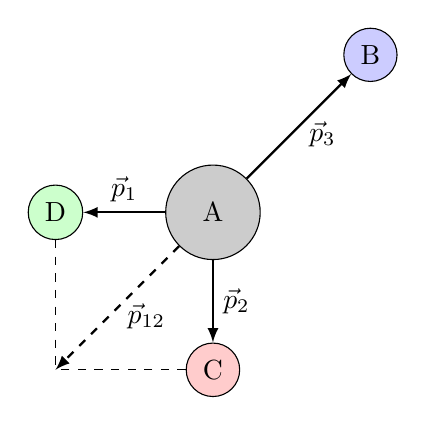
\begin{tikzpicture}
		\node[circle, draw, fill=black!20, minimum size = 1.2cm] (A) at (0,0) {A};
		\node[circle, draw, fill=blue!20] (B) at (2,2) {B};
		\node[circle, draw, fill=red!20] (C) at (0,-2) {C};
		\node[circle, draw, fill=green!20] (D) at (-2,0) {D};

		\draw[-latex, thick] (A)-- node[right, yshift=-0.1cm]{$\vec{p}_3$} (B);
		\draw[-latex, thick] (A)-- node[right]{$\vec{p}_2$} (C);
		\draw[-latex, thick] (A)-- node[above]{$\vec{p}_1$} (D);
		\draw[-latex, dashed, thick] (A) -- node[right, yshift=-0.1cm]{$\vec{p}_{12}$}(-2,-2);
		\draw[dashed] (C) -- (-2,-2);
		\draw[dashed] (D) -- (-2,-2);
	\end{tikzpicture}
	\caption{Schema del decadimento in tre corpi nel sistema del centro di massa}
	\label{fig:decadimento_tre_corpi}
\end{figure}

Nel sistema del centro di massa valgono le seguenti relazioni (la particella
che decade nel sistema del centro di massa ha impulso nullo):
\begin{equation}
	\begin{dcases}
		\vec{p}_1 + \vec{p}_2 + \vec{p}_3 = 0
		\\
		\varepsilon_1 + \varepsilon_2 + \varepsilon_3 = E ^{\ast} = M
	\end{dcases}
	\label{eq:sistema_tre_corpi}
\end{equation}
Per risolvere il problema lo riduciamo in un decadimento in due corpi
introducendo la \textit{particella virtuale}\footnote{
	Il ragionamento può essere applicato a ognuna delle particelle per
	permutazione delle coppie
} $\boldsymbol{DC}$ di massa $M_{12} = m_1 + m_2$, tale che
$M = M _{12} + m_3$, e d'impulso $\vec{p}_{12} = \vec{p}_1 + \vec{p}_2$.
Il quadrimpulso della particella $\boldsymbol{DC}$ sarà la somma dei
quadrimpulsi delle singole particelle:
\begin{equation}
	\qvec{P}_{12}
	= \qvec{P}_1 + \qvec{P}_2
	= \Set{\eps_1 + \eps_2, \vec{p}_1 + \vec{p}_2}
\end{equation}
L'invariante relativistico associato:
\begin{equation}
	M_{12}^2 = \qvec{P}_{12}^2 = \mrb{\eps_1 + \eps_2}^2 -
	\mrb{\vec{p}_1 + \vec{p}_2}^2
\end{equation}
Osserviamo che $M_{12}$ non è costante, ma varia nei limiti cinematici imposti
dalla conservazione del quadrimpulso.
Risolvendo le equazioni \ref{eq:sistema_tre_corpi} per la particella $B$
otteniamo:
\begin{equation}
	M_{12}^2
	= \mrb{M - \eps_3}^2 - \abs{\vec{p}_3}^2
	= M^2 + m_3^2 - 2 M \eps_3
\end{equation}
\begin{equation}
	\Rightarrow \boxed{
		\eps_3 = \frac{M^2 + m_3^2 - M_{12}^2}{2 M}
	}
	\label{eq:epsilon_tre}
\end{equation}
Dall'ultima equazione è evidente come $\eps_3$ dipenda dal valore di
$M_{12}$. Quindi possiamo trovare gli estremi di $\eps_3$, ovvero
$\mrb{\eps_3}_{\text{min}}$ e $\mrb{\eps_3}_{\text{max}}$.

\begin{note}[]
	Possiamo ripetere il ragionamento per per trovare
	$\mrb{\eps_i}_{\text{min,max}}, \forall i = 1, 2, 3$.
\end{note}

\subsection{Energia minima}
La condizione per cui $\eps_3 = \mrb{\eps_3}_{min}$ è che la
particella $\boldsymbol{B}$ sia emessa a riposo rispetto al sistema del centro
di massa\footnote{
	Questa condizione è \textit{cinematicamente ammissibile}
}. Infatti in tale condizione:
\begin{equation}
	\begin{dcases}
		\mrb{\vec{p}_3}_{min} = 0
		\\
		\mrb{\eps_3}_{min} = m_3
	\end{dcases}
\end{equation}
l'energia corrisponde alla massa a riposo (che è l'energia minima che una
particella possa assumere). Dall'equazione \ref{eq:epsilon_tre} otteniamo un
valore per $M_{12}$ in condizione di energia minima per la particella
$\boldsymbol{B}$:
\begin{equation}
	\eps_3 = \frac{M^2 + m_3^2 - M_{12}^2}{2 M} = m_3
\end{equation}
Quindi:
\begin{equation}
	M_{12}^2 =  M^2 + m_3^2 - 2 M m_3 = \mrb{M - m_3}^2
\end{equation}
\begin{equation}
	\Rightarrow \boxed{M_{12} = M - m_3}
\end{equation}
Calcoliamo anche $\abs{\vec{p}\,} = \abs{\vec{p}_1} = \abs{\vec{p}_2}$ relativo
a questa configurazione del sistema:
\begin{equation}
	\begin{dcases}
		\vec{p}_1 + \vec{p}_2 = 0
		\\
		\eps_1 + \eps_2 = M - m_3
	\end{dcases}
\end{equation}
quindi si ricava:
\begin{equation}
	\boxed{
		\abs{\vec{p}}
		= \abs{\vec{p}_1}
		= \abs{\vec{p}_2}
		= \frac{
			\msb{\mrb{M - m_3}^2 - \mrb{m_1 + m_2}^2}
			\msb{\mrb{M - m_3}^2 - \mrb{m_1 - m_2}^2}
		}{4 \mrb{M - m_3}^2}
	}
\end{equation}

\subsection{Energia massima}
Come si può osservare dall'equazione \ref{eq:epsilon_tre}, il valore massimo di
energia $\eps_3$ si ottiene in corrispondenza del valore minimo della
massa invariante $M_{12}$ della particella fittizia $\boldsymbol{DC}$\footnote{
	Sempre in riferimento alla figura \ref{fig:decadimento_tre_corpi}
}.
\begin{equation}
	\mrb{M_{12}}_{\text{min}} \longrightarrow \mrb{\eps_3}_{\text{max}}
\end{equation}
Quindi, scrivendo esplicitamente $M_{12}$:
\begin{align}
	M_{12}^2
	 & = \mrb{\eps_1 + \eps_2}^2 - \mrb{\vec{p}_1 + \vec{p}_2}^2
	\\\notag
	 & = \eps_1^2 + \eps_2^2 + 2 \eps_1 \eps_2 - \abs{\vec{p_1}}^{2} -
	\abs{\vec{p}_{2}}^{2} - 2 \vec{p}_{1} \cdot \vec{p}_{2}
	\\\notag
	 & = m_1^2 + m_2^2 + 2 \mrb{\eps_1 \eps_2 - \vec{p}_1 \cdot
		\vec{p}_2}
\end{align}
quindi, poiché $m_1$ ed $m_2$ sono costanti, $M_{12}$ è minimo quando è minima
la quantità in parentesi. E al minimo la quantità in parentesi vale proprio
$m_1 m_2$. Questa condizione coincide con la configurazione in cui le due
particelle $\boldsymbol{C}$ e $\boldsymbol{D}$ vengono emesse a riposo.
La precedente equazione diventa:
\begin{equation}
	M_{12}^2 \geq \mrb{m_1 + m_2}^2
\end{equation}
e l'uguaglianza \textit{stretta} è rispettata se le due particelle
$\boldsymbol{C}$ e $\boldsymbol{D}$ si muovono nella stessa direzione e con la
stessa velocità, ovvero quando valgono le seguenti condizioni:
\begin{equation}
	\frac{\vec{p}_1}{\eps_1} = \frac{\vec{p}_2}{\eps_2}
	\msse
	\vec{\beta}_1 = \vec{\beta}_2 =\vec{\beta}
\end{equation}

Si verifica, infatti, che sostituendo nell'espressione di $M_{12}^2$
(utilizziamo la relazione $\gamma = \frac{E}{m}$):
\begin{align}
	M_{12}^2
	 & = m_1^2 + m_2^2 + 2 \mrb{\eps_1 \eps_2 - \vec{p}_1 \cdot
		\vec{p}_2}
	\\\notag
	 & = m_1^2 + m_2^2 + 2 \mrb{\eps_1 \eps_2 -
		\beta_1\eps_1 \beta_2\eps_2}
	\\\notag
	 & = m_1^2 + m_2^2 + 2 \eps_1 \eps_2 \mrb{1 - \beta_1 \beta_2}
	\\\notag
	 & = m_1^2 + m_2^2 + 2 \eps_1 \eps_2 \mrb{1 - \beta^2}
	\\\notag
	 & = m_1^2 + m_2^2 + 2 \eps_1 \eps_2 \frac{1}{\gamma^2}
	\\\notag
	 & = m_1^2 + m_2^2 + 2 m_1 \cancel\gamma m_2 \cancel\gamma
	\frac{1}{\cancel\gamma^2}
	\\\notag
	 & = m_1^2 + m_2^2 + 2 m_1 m_2
	\\\notag
	 & = \mrb{m_1 + m_2}^2
\end{align}

Possiamo quindi concludere che:
\begin{equation}
	\boxed{
		\mrb{\eps_3}_{max} = \frac{M^2 + m_3^2 - \mrb{m_1 + m_2}^2}{2M}
	}
\end{equation}

\begin{example}[Decadimento $\beta^-$]
	Vogliamo calcolare l'intervallo di energia permesso all'elettrone nel
	decadimento $\beta^-$ (reazione frequente all'interno dei nuclei atomici):
	\begin{equation}
		n \rightarrow p + e^- + \cc{\nu}_{e}
	\end{equation}
	\textit{Essendo un decadimento a tre corpi, non esiste un'energia ben
		definita per l'elettrone.}
	Le masse delle particelle sono:
	\begin{equation}
		m_n = \qty{939.56}{\MeV \per c^2};
		\qquad
		m_p = \qty{938.27}{\MeV \per c^2};
		\qquad
		m_e = \qty{0.511}{\MeV \per c^2};
		\qquad
		m _{\cc{\nu}} \simeq \qty{0}{\MeV \per c^2}
	\end{equation}
	Quindi le energie per l'elettrone, a reazione avvenuta:
	\begin{equation}
		\begin{dcases}
			\mrb{\eps_{e^-}}_\text{min} = m_{e^-} = \qty{0.511}{\MeV}
			\\
			\mrb{\eps_{e^-}}_\text{max}
			= \frac{m_n^2 + m_{e^-}^2 - m_p^2}{m_{e^-}^2}
			\simeq \qty{1.3}{\MeV}
		\end{dcases}
	\end{equation}
\end{example}

\begin{example}[Decadimento del muone]
	Vediamo ora la reazione di decadimento del muone $\mu^+$:
	\begin{equation}
		\mu^+ \rightarrow e^+ + \nu_e + \cc{\nu}_{\mu}
	\end{equation}
	dove $e^+$ è un \textit{positrone}, $\nu_e$ è un \textit{neutrino elettronico}
	e $\cc{\nu}_{\mu}$ un \textit{antineutrino muonico}.
	Le masse sono:
	\begin{equation}
		m _{\mu^+} = \qty{105.7}{\MeV \per c^2};
		\qquad
		m _{\cc{\nu}_{\mu}} = m _{\nu_e} = 0;
		\qquad
		m_{e^+} = \qty{0.511}{\MeV \per c^2}
	\end{equation}
	Quindi le energie:
	\begin{equation}
		\begin{dcases}
			\mrb{\eps_{e^+}}_\text{min} = m_e^+ = \qty{0.511}{\MeV}
			\\
			\mrb{\eps_{e^+}}_\text{max}
			= \frac{m _{\mu}^{2} + \cancel{m_{e^+}^2}}{2 m_{\mu^+}}
			\simeq \frac{m _{\mu^+}}{2}
			= \qty{52.8}{\MeV}
		\end{dcases}
	\end{equation}
\end{example}

\begin{example}[]
	Vediamo un ultimo esempio\footnote{
		La particella $\omega$ è un \textbf{mesone}
	}:
	\begin{equation}
		\omega \rightarrow \pi^+ + \pi^- + \pi^0
	\end{equation}
	Le masse sono:
	\begin{equation}
		m _{\omega} = \SI{782}{\MeV \per c^2};
		\qquad
		m _{\pi} = \SI{140}{\MeV \per c^2}
	\end{equation}
	Le energie:
	\begin{equation}
		\begin{dcases}
			\mrb{\eps _{\pi}}_\text{min} = m _{\pi} = \SI{140}{\MeV}
			\\
			\mrb{\eps _{\pi}}_\text{max} = \frac{m _{\omega}^{2} + m _{\pi}^{2} - 4 m
					_{\pi}^{2}}{2 m _{\omega}} = \frac{m _{\omega}^{2} - 3 m _{\pi}^{2}}{2 m
					_{\omega}} = \SI{353}{\MeV}
		\end{dcases}
	\end{equation}
\end{example}
